\begin{figure}[!htb]
	\begin{subfigure}{.5\linewidth}
		\centering
		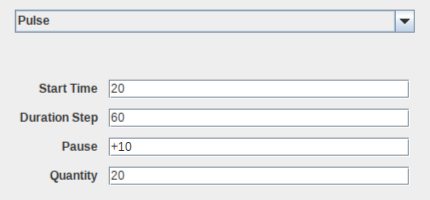
\includegraphics[scale=0.7]{condiguracao-carga-modulada1.png}
		\caption{Carga gerada com base na configuração}
		\label{fig:sub1}
	\end{subfigure}%
	\begin{subfigure}{.5\linewidth}
		\centering
		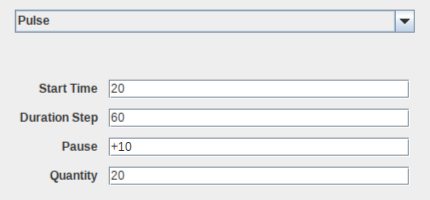
\includegraphics[scale=0.7]{condiguracao-carga-modulada1.png}
		\caption{Carga gerada com base na configuração}
		\label{fig:sub2}
	\end{subfigure}\\[1ex]
	\begin{subfigure}{\linewidth}
		\centering
		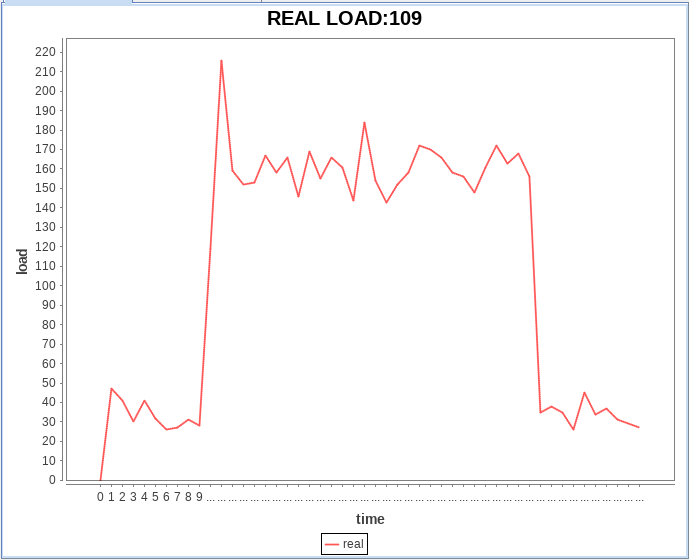
\includegraphics[scale=0.6]{grafico-carga-modulada1.png}
		\caption{Carga gerada com base na configuração}
		\label{fig:grafico-carga-modulada}
	\end{subfigure}
	\caption{Carga gerada com base na configuração}
	\label{fig:test}
	\fautor
\end{figure}



\begin{figure}[!htb]
	\begin{subfigure}{.5\linewidth}
		\centering
		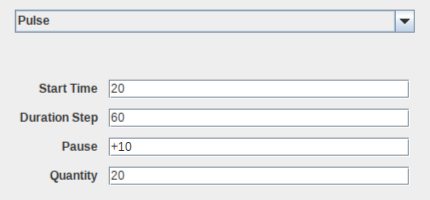
\includegraphics[scale=0.7]{condiguracao-carga-modulada1.png}
		\caption{onda quadrada}
		\label{fig:sub1}
	\end{subfigure}%
	\begin{subfigure}{.5\linewidth}
		\centering
		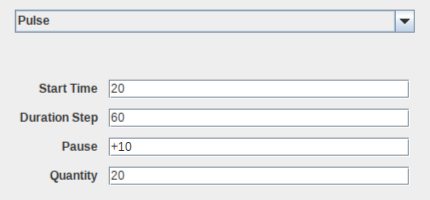
\includegraphics[scale=0.7]{condiguracao-carga-modulada1.png}
		\caption{onda quadrada}
		\label{fig:sub2}
	\end{subfigure}\\[1ex]
	\begin{subfigure}{\linewidth}
		\centering
		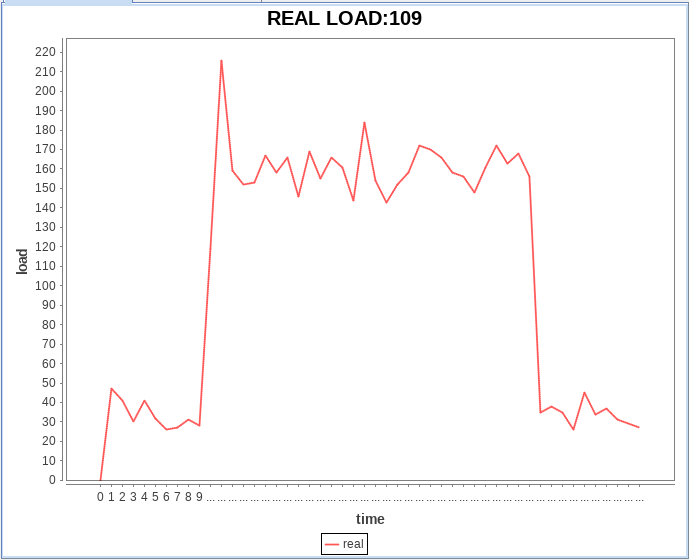
\includegraphics[scale=0.6]{grafico-carga-modulada2.png}
		\caption{onda quadrada}
		\label{fig:grafico-carga-modulada}
	\end{subfigure}
	\caption{onda quadrada}
	\label{fig:test}
	\fautor
\end{figure}

\begin{figure}[!htb]
	\begin{subfigure}{.5\linewidth}
		\centering
		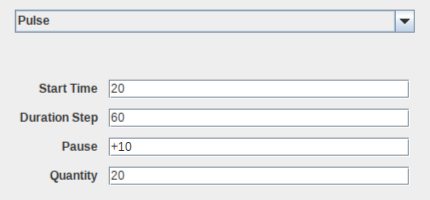
\includegraphics[scale=0.7]{condiguracao-carga-modulada1.png}
		\caption{Degrau negativo}
		\label{fig:sub1}
	\end{subfigure}%
	\begin{subfigure}{.5\linewidth}
		\centering
		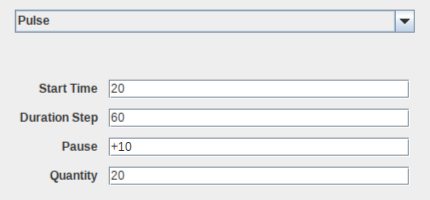
\includegraphics[scale=0.7]{condiguracao-carga-modulada1.png}
		\caption{Degrau negativo}
		\label{fig:sub2}
	\end{subfigure}\\[1ex]
	\begin{subfigure}{\linewidth}
		\centering
		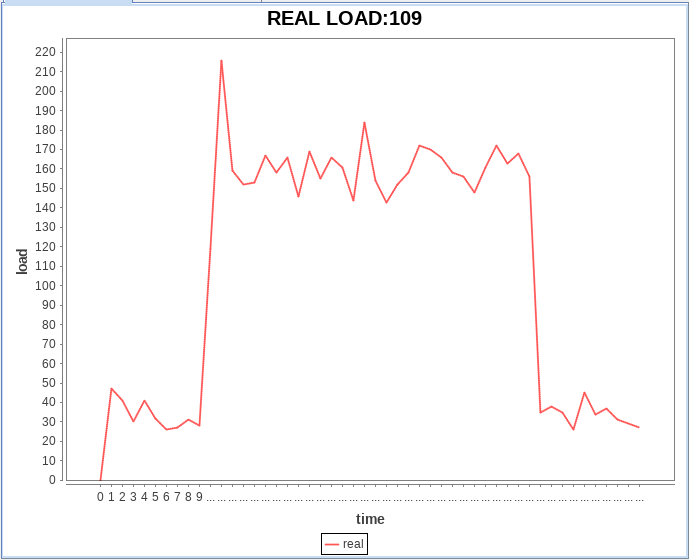
\includegraphics[scale=0.6]{grafico-carga-modulada2.png}
		\caption{Degrau negativo}
		\label{fig:grafico-carga-modulada}
	\end{subfigure}
	\caption{Degrau negativo}
	\label{fig:test}
	\fautor
\end{figure}


%3º  - mostrar a analise e o impacto do carga de trabalho no sistema  
%Podemos agora usar os resultados da análise de desempenho para atender as metas estabelecidas no ponto 6.3.1. Por meio do modelo de QPN desenvolvido, que foram capazes de prever o desempenho do sistema em condições de funcionamento normais com 4 e 6 servidores WebLogic. Descobriu-se que usando o balanceador de carga original, seis nós de servidor de aplicação não foram suficientes para garantir tempos médios de resposta de transações de negócios abaixo de meio segundo. Atualizando o balanceador de carga com um CPU ligeiramente mais rápido levou à utilização de CPU do dropping balanceador de carga por um bom 20 por cento.
%Como resultado, os tempos de resposta de transações de concessionários melhorou em 15 a 27 por cento, encontrando o "meio segundo" exigência. No entanto, o aumento da intensidade da carga de trabalho além das condições de pico revelou que o balanceador de carga foi um recurso gargalo, impedindo-nos para escalar o sistema adicionando servidores WebLogic adicionais (veja a Figura 6.14). Assim, à luz do crescimento da carga de trabalho que o esperado, a empresa deve substituir a máquina balanceador de carga com um mais rápido ou considerar o uso de um método de balanceamento de carga mais eficiente. Depois de feito isso, a análise de desempenho deve ser repetida com o novo balanceador de carga para se certificar de que não há nenhum outro gargalos do sistema. Também deve ser assegurado que o balanceador de carga é configurado com threads suficientes para que não há contenção de discussão.
%Neste capítulo, a prática metodologia de modelagem de desempenho para DCS foi apresentada.
%A metodologia aproveita o poder de modelagem e expressividade do formalismo de modelagem QPN para melhorar a representatividade do modelo e permitir a previsão de desempenho precisas. Foi apresentado um estudo de caso detalhado no qual um modelo de um DCS realista foi construído e usado para analisar o seu desempenho e escalabilidade.
%O modelo de representatividade foi validado comparando suas previsões contra medições no sistema real. Foram considerados Um número de diferentes configurações de implantação e cenários de carga de trabalho. Além disso a CPU e I / O de contenção, demonstrou-se como alguns aspectos mais complexas do comportamento do sistema, tais como a contenção de rosca e processamento assíncrono, pode ser modelado. O modelo mostrou para refletir com precisão as características do sistema de desempenho e escalabilidade em estudo. O erro de modelagem para o tempo de resposta da transação não ultrapassou 21,2% e foi muito menor para a transferência de transações e utilização de recursos. A metodologia de modelagem de desempenho proposto fornece uma ferramenta poderosa para a engenharia de DCS desempenho.

1-Projete o protocolo de estudo de caso:
	a - determinar as competências necessárias
	b - desenvolver e revisar o protocolo

2-Conduta do estudo de caso:
	a - preparar-se para a coleta de dados
	b - distribuir questionário
	c - realizar entrevistas

3 Analisar caso provas estudo:
	a - analítica estratégia

4-Desenvolver conclusões, recomendações, e as implicações com base nas provas

%As análises apresentadas nessa Seção consideram a execução de rajadas de requisições dos usuários com e sem a presença de mecanismos de segurança, seguindo o planejamento definido na Seção anterior. Dessa forma, para uma melhor abordagem dos dados analisados, as avaliações foram divididas em duas Seções de acordo com o cenário.

\section{Contribuição}